\documentclass{scrbook}
\usepackage[ngerman, main=english]{babel}
\usepackage{fontspec}

\usepackage{amsmath}
\usepackage{mathrsfs}
\usepackage{csquotes}
\usepackage{amssymb}
\usepackage{float}
\usepackage{hyperref}
\usepackage{cleveref}
\usepackage{nicefrac}
\usepackage[toc, page]{appendix}
\usepackage{subcaption}
\usepackage{caption}
\usepackage{booktabs}
\usepackage{textcomp}
\usepackage{makecell}
\usepackage[export]{adjustbox}
\usepackage{pict2e}
\usepackage{tikz}
\usetikzlibrary{%
    decorations.pathreplacing,%
    decorations.pathmorphing%
}
\usepackage[european]{circuitikz}
\usepackage{xcolor}
\usepackage{pgfornament}
\captionsetup[subfigure]{labelfont=bf,labelformat=simple,textfont=normalfont,singlelinecheck=off,justification=raggedright}
 \renewcommand{\thesubfigure}{\Alph{subfigure}}
\usepackage{scalerel}
\newcommand{\myequation}{\begin{equation}}
\newcommand{\myendequation}{\end{equation}}
\let\[\myequation
\let\]\myendequation

\newcommand{\red}[1]{\textcolor{red}{#1}}
\newcommand{\hbn}{{\footnotesize h}\textsc{bn}}
\newcommand{\hbng}{{\footnotesize h}\textsc{bn}\ }
\newcommand{\tmd}{\textsc{tmd}}
\newcommand{\tmdg}{\textsc{tmd}\ }
\newcommand{\tmds}{\textsc{tmd}s\ }
\newcommand{\pdms}{\textsc{pdms}}
\newcommand{\ppc}{\textsc{ppc}}
\newcommand{\si}{\textsc{s}i}
\newcommand{\sio}{\textsc{s}i\textsc{o}$_{\scaleto{2}{4pt}}$\ }
\newcommand{\ws}{\textsc{w}\textsc{s}$_{\scaleto{2}{4pt}}$\ }
%\newcommand{\wse}{\textsc{w}\textsc{s}{\footnotesize e}$_{\scaleto{2}{4pt}}$\ }
\newcommand{\wse}{\textsc{w}\textsc{s}e$_{\scaleto{2}{4pt}}$\ }
\newcommand{\mos}{\textsc{m}o\textsc{s}$_{\scaleto{2}{4pt}}$\ }
\newcommand{\mose}{\textsc{m}o\textsc{s}e$_{\scaleto{2}{4pt}}$\ }
\newcommand{\pl}{\textsc{pl}\ }
\newcommand{\mbeq}{\overset{!}{=}}
\newcommand{\sigp}{\sigma$^+$}
\newcommand{\sigm}{\sigma$^-$}

\renewcommand{\arraystretch}{1.2}

\usepackage{mathpazo}
%\setsansfont{[futura_medium_bt.ttf]}
%\setmainfont[
% BoldFont={[Futura_Bold_font.ttf]}, 
% ItalicFont={Futura_Light_Italic_font.ttf},
% BoldItalicFont={[Futura_Bold_Italic_font.ttf]}
% ]{[futura_light_bt.ttf]}
\setmainfont[Numbers={Proportional,OldStyle}]{Linux Libertine O}
\setkomafont{sectioning}{\scshape\addfontfeatures{Numbers=Lining}}
\setkomafont{title}{\scshape}
%\setkomafont{section}{\rmfamily}

\usepackage{graphicx}
\usepackage{caption}
\usepackage{subcaption}
\usepackage[backend=biber,style=phys,sorting=none,natbib=true]{biblatex}
\addbibresource{literature.bib}
\usepackage{remreset}

\renewcommand{\autodot}{}
\newcommand{\titleen}{Earth is flat\\ and the sun is cold}
\newcommand{\titlede}{Shooting some lasers\\ to disprove the lizard overlords}
%\newcommand{\titleen}{Spectroscopy of gate-tunable\\ thin films of tungsten-diselenide}
%\newcommand{\titlede}{Spektroskopie ladungsdurchstimmbarer dünner schichten aus wolfram-diselenid einzellagen}
\title{Spectroscopy of gate-tunable tungsten-diselenide monolayers}
\subtitle{Master's Thesis}
\author{Jonathan Förste}

\begin{document}
%\maketitle
%\begin{titlepage} % Suppresses headers and footers on the title page

	\centering % Centre everything on the title page
	
	\scshape % Use small caps for all text on the title page
	
	\vspace*{\baselineskip} % White space at the top of the page
	
	%------------------------------------------------
	%	Title
	%------------------------------------------------
	
	\rule{\textwidth}{1.6pt}\vspace*{-\baselineskip}\vspace*{2pt} % Thick horizontal rule
	\rule{\textwidth}{0.4pt} % Thin horizontal rule
	
	\vspace{0.75\baselineskip} % Whitespace above the title
	
	{\LARGE \textsc{\titleen}\\\pgfornament[width = 4cm,
color = black]{89}\\\vspace{0.3cm}\titlede\\} % Title
	
	\vspace{0.75\baselineskip} % Whitespace below the title
	
	\rule{\textwidth}{0.4pt}\vspace*{-\baselineskip}\vspace{3.2pt} % Thin horizontal rule
	\rule{\textwidth}{1.6pt} % Thick horizontal rule
	
	\vspace{2\baselineskip} % Whitespace after the title block
	
	%------------------------------------------------
	%	Subtitle
	%------------------------------------------------
	Master's Thesis % Subtitle or further description
	
	\vspace*{3\baselineskip} % Whitespace under the subtitles
	
	%------------------------------------------------
	%	Editor(s)
	%------------------------------------------------
	
	By
	
	\vspace{0.5\baselineskip} % Whitespace before the editors
	
	{\scshape\Large Jonathan Förste \\} % Editor list

	\vspace{10\baselineskip} % Whitespace below the editor list %10
	
	supervised by

	\vspace{0.3\baselineskip} % Whitespace before the editors

	{\scshape\Large Prof. Dr. Alexander Högele \\} % Editor list
	%{\scshape\Large Dr. Axel Stoll \\}

	\vspace{0.5\baselineskip}

	Faculty of Physics --- Nano-Photonics Group
	%Promovierter Naturwissenschaftler

	\vspace{0.5\baselineskip}

	\textit{Ludwig-Maximilian-Universität \\ München} % Editor affiliation
	%\textit{Neuschwabenland Forum \\ München}	

	\vfill % Whitespace between editor names and publisher logo
	
	%------------------------------------------------
	%	Publisher
	%------------------------------------------------
	
	%\plogo % Publisher logo
	
	\vspace{0.3\baselineskip} % Whitespace under the publisher logo
	
	\today% Publication year
	

\end{titlepage}

%\addchap*{Abstract}
%Legal disclaimer: This thesis contains more bullshit than the \textsc{eu-bsgvo} allows. Children, elderly people and pregrant women therefore are not allowed to read beyond this abstract and should consult a doctor if they experience the desire to facepalm for more than two consecutive days.\newline

Two dimentional semiconductors made of transition metal dichalchogenides (\tmds\!) have attracted a lot of interest because of their unique optical and electrial properties like a direct band gap, strong spin-orbit coupling, valley polarization and a high exciton binding energy. Optical spectroscopy of these materials has however been limited by inhomogneious broadening of spectral lines related to charge defects in the dielectric environment. Also, their varying degrees of intrinsic unintentional doping have made comprehensive studies of the reflection and photoluminescence impossible without external control over the density of free charge carriers. Both of these issues have been tackled during the course of this master's thesis. Using high quality \hbng as a substrate results in narrow linewith \pl\ spectra and the electric contacting to a lithographicly written gold-structure gives rise to gate-tunability. Confocal spectrocopy of a sample of \wse both in the neutral and negative regime at different magnetic fields helps to identify previously misunderstood features.\newline
\begin{center}
\par\rule[8pt]{0.7\textwidth}{0.5pt}
\end{center}
Die besonderen optischen und elektronischen Eigenschaften zweidimensionaler Halbleiter aus einzelnen Schichten von Übergangsmetall-dichalgogeniden (\tmds\!) machen diese Materialien zu interessanten Forschungsobjekten. Die Kombination aus einer direkten Bandlücke im sichtbaren Bereich sowie einer starke Spin-Bahn-Kopplung, Valley-Polarisation und einer hohe Exziton Bindungsenergie ist einzigartig. Allerdings wird die Untersuchung dieser Systeme durch optische Spektroskopie durch Ladungsdefekte in der dielektrischen Umgebung erschwert, da Spektrallinien dadurch inhomogen verbreitert werden. Auch die intrinsische Dotierung, die von Probe zu Probe variieren kann macht ein vollständiges Verständnis des Spektrums ohne externe Kontrolle der Ladungsdichte unmöglich. In dieser Arbeit werden diese beiden Aspekte angegriffen: Um eine defektfreie dielektrische Umgebung zu schaffen, werden die Proben in hexagonales Bornitrid eingebettet und mit lithographischen Goldstrukturen kontaktiert um die Ladungsdichte durch den Feldeffekt zu steuern. In konfokaler Spektroskopie wird das neutrale und negativ geladene Spektrum einer \wse\!-Probe untersucht und das Verhalten der Spektrallinien im Magnetfeld beobachtet um bisher unverstandene Lininen zu identifizieren.
%\tableofcontents
\chapter{Introduction}
Ever since Andre Geim and Konstantin Novoselov were awarded the Nobel prize for their discovery of graphene, two-dimensional materials have become a centerpiece of condensed matter physics. After graphene, a lot of 2\textsc{d} materials were found, that each 
\cite{langer_lightwave_2018}
%\chapter{Physical properties of thin film transition metal dichalcogenides}

\section{Crystal structure and symmetries}

\begin{figure}[t]
	\centering
	\begin{subfigure}{0.30\textwidth}
		\caption{}
		\includegraphics[height=.9\textwidth,left]{3d}
		\label{crystal1}
	\end{subfigure}
	\begin{subfigure}{0.30\textwidth}
		%\centering
		\caption{}
		\includegraphics[height=.9\textwidth,center]{triangles}
		\label{crystal2}
	\end{subfigure}
	\begin{subfigure}{0.30\textwidth}
		\centering
		\caption{}
		\includegraphics[height=.9\textwidth,right]{topview}
		\label{crystal3}
	\end{subfigure}
	\caption{Crystal structure of \tmds\!: \textbf{A} \tmds are composed of large sheets of transition metal atoms sandwiched in between chalcogenite atoms. Individual sheets are bound by strong in-plane covalent bonds and are being held together out-of-plane only by weak van-der-Waals forces. \textbf{B} In the 2\textsc{h} phase, the unit cell of \tmds has a triagonal prismatic shape with the transition metal in the center, between two triangles of chalcogenite atoms. \textbf{C} Viewed from the top, \tmds show a hexagonal lattice structure. However, because of the structure of the unit cell, the inversion symmetry is broken. Graphics from \cite{wang_electronics_2012, xiao_coupled_2012}}\label{crystal}
\end{figure}

Transition metal dichalcogenides (\tmds\!) belong to a class of materials that consist of large covalently bound sheets, that are held together by weak van-der-Waals forces. These so-called layered materials have gotten more attention since it has been shown, that individual monoatomic layers of them have unique properties, that are very different from the bulk material. The most prominent member of this group is graphene. Graphenes band structure shows what is called "dirac cones". This means that conduction and valence band touch at the $K$ point at the edge of the Brilloin zone, with the Fermi level seperating the two. The electronic dispersion relation in the vicinity of these "Dirac points" is linear. As a result charge carriers like electrons effectively behave like massless fermions, analogously to the linear dispersion of photons. This among other things causes very high electron mobility and conductivity. \textsc{Tmdc}s on the other hand are semiconductors and have long been known to have an indirect band gap. However, only since the discovery of graphene their properties in the limit of one atomic sheet---the monolayer---came into focus. Crystals of \tmds consist of a tri-atomic base of one transition metal atom like tungsten (W) or molybdenum (Mo) and two chalcogen atoms like sulfur (S), selenium (Se) or tellurium (Te). In nature these compounds can be found in lateral arrangement---a \tmdg monolayer (see figure \ref{crystal} \textbf{A}). \textsc{Tmd}s can exist in different metastable phases, that have a different crystal structure as well as different electronic properties \cite{ouyang_phase_2015}. The stable semiconducting phase is called 2\textsc{h}. In this configuration every transition-metal atom has six neighboring chalcogen atoms and forms a trigonal prismatic unit-cell, with the transition-metal in the center as depicted in figure \ref{crystal} \textbf{B}. A \tmdg monolayer exhibits a $\mathcal{D}^1_{3h}$-symmetry. The unit-cell is invariant under 3-fold rotation as well as in-plane reflection. In the top-view (see figure \ref{crystal} \textbf{C}) this looks similar to the hexagonal lattice structure of graphene, but with the key difference of a broken inversion symmetry. When the unit-cell is inverted with the transition metal atom as its inversion center, the chalcogen atoms wind up in empty locations as with any possible inversion point.

This has two important consequences, regarding the electronic band structure. As in graphene, the reciprocal lattice is hexagonal. At the $K$ points however, instead of the characteristic dirac cone, monolayer \tmds form a direct band gap in the visible range. Because of inversion symmetry breaking the degeneracy of the $K$ points is lifted. The two different $K$ and $K'$ points that are identical in graphene are distinguishable in \tmds and exhibit optical selection rules, coupling the valleys to light with opposite helicity. This circular dichroism gives rise to a new pseudo-spin degree of freedom---the "valley index". Analogous to electronics and spintronics, the term ``valleytronics'' has been coined to describe possible information processing by manipulating this property \cite{wang_electronics_2012, xiao_coupled_2012}. 

The valence and conduction bands of \tmds are formed by the hybridization of the $d$-orbitals of the transition metal with the $p$-orbitals of its six neighboring chalcogen atoms. More precisely, the first four conduction bands and the seven first valence bands are dominated by the five 5$d$ (4$d$) and 4$p$ (3$p$) orbitals of W (Mo) and Se (S) respecively, carrying 93\% of the total orbital weight \cite{cappelluti_tight-binding_2013,silva-guillen_electronic_2016}. At the $K$ and $K'$ points the valence band is formed mainly by the $d_{x^2-y^2}$ and $d_{xy}$ orbitals of the metal atom, that leads to large spin-orbit coupling that splits the valence bands by more than 150 meV  \cite{zhu_giant_2011}. This energy is large enough to suppress any transition between the two valence subbands even at room temperature. Because of time-reversal symmetry, the splitting is reversed in the $K'$ valley. With regards to optical transitions this results in tight locking of spin and valley degree of freedom. The conduction band---formed by the $d_{z^2}$ orbtial of the metal with some contribition from $p_x$ and $p_y$ of the chalcogen---exhibits much weaker but finite spin-orbit splitting, that leads to two distinct optical transitions $X$ and $D$, that will be explained later on.

\section{Excitons in \tmdg monolayers}\label{theory_exciton}

When electrons absorb photons of an energy higher than the band gap of a semiconductor, they gain enough energy to be elevated to the conduction band and are allowed to move freely throughout the crystal. Other electrons can hop to the vacancies making the holes just as free as excited electrons. They also effectively act like a positive charges, resulting in Coulomb forces between free electrons and holes. If this interaction is strong enough to overcome thermal excitation, the two quasiparticles can enter a bound state, called ``exciton''. In a bulk semiconductor electrons in between electron and hole weaken this interaction by screening the Coulomb interaction which results in a low exciton binding energy. The direct semiconductor \textsc{g}a\textsc{a}s for example exhibits an exciton binding energy of just 4.2 meV \cite{pelant_luminescence_2012}. Doing a rough calculation with $T=E_{binding}/k_B$ this corresponds to a temperature of 48 K, limiting exciton formation to temperatures well below that of liquid nitrogen.
The geometry of \tmdg monolayers however effectively reduces the screening effect. Because the movement of electrons and holes is confined to two dimensions, the electric field density in the material drops significantly and the strong Coulomb interaction between the free quasiparticles raises the exciton binding energy up to several hundred meV \cite{chernikov_exciton_2014, hanbicki_measurement_2015, he_tightly_2014}, corresponding to several thousand K in temperature. Therefore excitons can be excited at room temperature, which raises the possibility of exciton-based real-life applications. The Coulomb interaction results in an exciton Bohr radius of close to 1 nm and a very short lifetime in the order of picoseconds \cite{palummo_exciton_2015}. Hence, the recombination of excitons with emission of a photon is the most efficient optical decay channel and thus dominates the photoluminescence spectrum.
The decay also happens much faster than the so called valley lifetime---the timescale of coupling between the valleys---preserving the helicity in their emission once they decay. This is called "valley polarization".
The thinness of \tmdg monolayers has additional implications. Since the electric dipole field of the exciton extends beyond the boundaries of the crystal, the dielectric environment has a big influence on the optical spectrum \cite{stier_probing_2016, borghardt_engineering_2017, jakubczyk_impact_2018}. Impurities such as microscopic water droplets or dangling bonds of silicon oxide can induce localized potentials, broadening the linewidth of the photoluminescence (\pl\!) features. This complicates spectroscopic studies. On the other hand, this high sensitivity could be used in quantum sensing applications to optically probe or visualize electric or magnetic proximity effects \cite{peng_valley_2017, zhao_enhanced_2017, smolenski_tuning_2016, neumann_opto-valleytronic_2017}.


\begin{figure}[t]
\centering
\includegraphics[width=.6\textwidth]{bandstructure}
\caption{Band structure for \mos and \wse mono- and bilayers calculated for room temperature. In the limit of a single atomic layer \tmds form a direct band gap at the $K$-point and the valence band is strongly split due to spin-orbit coupling. Graphic taken from  \cite{zibouche_transition-metal_2014_2}.}
\label{bandgap}

\end{figure}

\section{Optical spectrum of ws\textup{e}$_2$ monolayers}\label{composition}

\begin{figure}[t]
\centering
\begin{subfigure}{0.69\textwidth}
	\caption{}
	\includegraphics[width=.8\textwidth]{Band_structure_momentum_dark}
\end{subfigure}
\begin{subfigure}{0.3\textwidth}
	\caption{}
	\begin{tabular}{@{}rrrrr@{}}
	\toprule
	Mode&\Gamma&K&Q\\
	\midrule
	TA&0&15.6&11.6\\
	LA&0&18.0&14.3\\
	TO(E')&30.5&26.7&27.3\\
	LO(E')&30.8&31.5&32.5\\
	A$_1$&30.8&31.0&30.4\\
	\bottomrule
	\end{tabular}
\end{subfigure}
\caption{\textbf{A} Diagram of the band structure of \mose and \wse\! \cite{lindlau_identifying_2017}. In contrast to \mose the spin-like bright transition ($X$) in \wse does not have the lowest energy. Because of spin-orbit coupling, the $K$ valley with opposite spin is lower in energy, as well as the $Q$ and $K$ valley with parallel spin components. As a result the population of spin-forbidden and momentum-indirect excitons could be high enough to enable significant contributions to the \pl spectrum by these states, whose radiative decay is less efficient. \textbf{B} The 3-atomic basis of \tmds results in 3 accoustic and 6 optical phonon modes. Of these only 2 accoustic and 3 optical modes can couple to charge carriers. For $QK$ and $KK'$ indirect excitons phonons in the $Q$- and $K$-valley supply the right momentum to enable an optical transition and the formation of phonon sidebands. Their energies are theoretically calculated in  \cite{jin_intrinsic_2014} and given in meV. }\label{phonon_band}
\end{figure}

As stated above, the optical spectrum of \tmds both in reflection and \pl is dominated by the decay of excitons. In Tungsten-diselenide (\wse\!) the \pl spectrum shows a rich ensemble of characteristic spectral features, that so far have not been identified unambiguously. 

For \hbng encapsulated \wse the main exciton resonance ($X$) is located at around 1.72 eV, but the precise value can shift several meV, mainly because of strain \cite{zhu_strain_2013}. This resonance corresponds to the creation and annihilation of an exciton in the $K$ valley with electron and hole having a parallel spin component. The corresponding exciton with antiparallel spins is often called the dark state as its ``spin-forbidden'' ($D$). For symmetry reasons\textregistered\ its radiative decay is only allowed in-plane and spin-orbit coupling puts the state about 40 meV lower than the bright exciton \cite{echeverry_splitting_2016}. The \pl from these excitons can be collected from the side or with a high numeric aperture objective, that catches light not directly emitted out-of-plane \cite{robert_fine_2017, wang_-plane_2017}. In the presence of free charges---either holes or electrons--- excitons can interact with them to form trions that are associated with a redshift of 20-30 meV \cite{courtade_charged_2017}. While these properties can be predicted by modeling the trion as a three-body quasi particle, its precise nature still remains under discussion. The most contrarian interpretation to the helium-like bound state is a so-called fermi polaron. In a charged regime excitons behave like an impurity in a ``sea'' of electrons, forming the polaron quasi particle \cite{sidler_fermi_2016, efimkin_many-body_2017,schmidt_fermi_2012}.

The spectrum of \wse shows additional features, that have so far escaped thorough understanding. In light of strong sample-to-sample variation, they are commonly attributed to localized effects, like defect-induced quantum dots or local doping \cite{kato_optical_2014, zhang_defect_2017}, that create trapped excitons. Improved fabrication techniques like mechanical exfoliation and the usage of \hbng as a substrate (see section \ref{exfoliation}) have enabled experimentalists to measure spectra with very little defects and narrow linewidths, that still show a rich class of reproducible features.

\subsection{Phonon sidebands}\label{sidebands}

These peaks can be identified as phonon side-bands of momentum-indirect excitons \cite{lindlau_identifying_2017}. It has been shown, that in contrast to molybdenum-based \tmds \wse actually shows an indirect band gap \cite{zhang_probing_2015, hsu_evidence_2017}. As can be seen in figure \ref{phonon_band} \textbf{A}, the $Q$-valley lies energetically close to the $K$-valley and is believed to be located lower than the upper $K$-valley, that participates in the direct spin-like exciton transition. This could point to a high population of excitons composed of electrons in the $Q$-valley as well as in the lower lying spin-like $K'$-valley. While both these states are spin-allowed, momentum conservation prevents them from radiatively decaying in a single-photon process. Instead they can recombine with assistance of an additional phonon, carrying the inter-valley momentum. For momentum conservation to hold, the following equations have to be fulfilled for momentum-indirect excitons in the $Q$- or $K'$-valley respectively:
\begin{align}
	\vec{k}_K + (\vec{k}_K - \vec{k}_{Q/K'}) &= \vec{k}_K + \vec{k}_{photon} + \vec{k}_{phonon}\\
	\Rightarrow \vec{k}_{phonon} &\mbeq \vec{k}_K - \vec{k}_{Q/K'}
\end{align}
with $\vec{k}_X$ being a reciprocal lattice vector with momentum $X$. Because of the hexagonal structure of the Brilloin zone $\vec{k}_K - \vec{k}_{K'}$ simply equals a phonon in $K$ while $\vec{k}_K - \vec{k}_{Q}$ is conveniently close to a phonon in $Q$. Crystal vibrations in \tmds can have three acoustic and six optical modes, but only two acoustic and three optical modes can couple to charge carriers. This leaves a total of five possible phonon sidebands for both $Q$- and $K'$-indirect excitons, neglecting processes involving more than one phonon. Corresponding theoretically calculated energies can be found in \ref{phonon_band} \textbf{B} \cite{jin_intrinsic_2014}. 

Phonon sidebands appear as a peak redshifted by these energy values. For $K'$-indirect excitons the positions of the peaks can be inferred directly, since the energy splitting between the spin-like and spin-unlike exciton is known and both features can be measured. The $Q$-valley however has no direct decay channel. Therefore, its energy has to be deduced from its sidebands.


% \cite{van_der_donck_excitons_2018} 

\section{The valley zeeman effect}\label{zeeman}

%\begin{figure}[t]
%\centering
%\begin{subfigure}{0.99\textwidth}
%	\begin{tikzpicture}
%	\node[above right] (img) at (0,0) {\includegraphics[width=\textwidth]{valleyzeeman}};
%	\node at (60pt, 160pt) {$E_S$};
%	\node at (140pt, 105pt) {$E_S$};
%	\node at (26pt, 160pt) {$E_{\mathrm{orb}}$};
%	\node at (340pt, 70pt) {$E_S$};
%	\node at (390pt, 155pt) {$E_S$};
%	\node at (390pt, 70pt) {$E_{\mathrm{orb}}$};
%	\node at (253pt, 200pt) {$K$};
%	\node at (165pt, 200pt) {$Q$};
%
%	\end{tikzpicture}
%\end{subfigure}
%\caption{Diagram of orbital and spin contributions to the valley Zeeman effect. For excitons with parallel spin, the corresponding shift $E_S$ of conduction and valence band cancels out. The shift for the direct spin-like exciton therefore depends mostly on the magnetic shift of the orbitals $E_{\mathrm{orb}}$ that at the $K$ point is non-vanishing only in the valence band. The spin-unlike direct exciton however has a strong spin contributioin which in theory doubles its $g$-factor. For momentum-indirect excitons in $Q$ the $g$-factor almost entirely due to the difference in effective mass between hole and electron, because both $E_S$ and $E_{\mathrm{orb}}$ shift in the same direction in the conduction and valence band.}
%	\label{flakes}
%\end{figure}

%\begin{figure}
%	%\centering
%	\resizebox{!}{70pt}{%
%	\begin{tikzpicture}[scale=0.32, every node/.append style={transform shape}]
%	\begin{circuitikz}
%		\draw (0, 0) parabola (4, 4);
%		\draw (0, 0) parabola (-4, 4);
%		\draw (10, 0) parabola (6, 4);
%		\draw (10, 0) parabola (14, 4);
%		\draw[line width=1mm, dash pattern=on 8pt off 6pt] (10, -2) parabola (6, 1.5);
%		\draw[line width=1mm, dash pattern=on 8pt off 6pt] (10, -2) parabola (14, 1.5);
%	\end{circuitikz}
%
%	\end{tikzpicture}
%	}
%	\caption{}
%\end{figure}

A splitting of spectral lines in presence of a magnetic field has been studied for over a hundred years and is called the Zeeman effect is named after the scientist first measuring it in the spectral lines of sodium. The shift of different energy levels in an atom is a result of the magnetic moment of the state, caused by its orbital angular momentum and spin. Solid crystals are large ensembles of atoms that merge atomic orbitals to form the electronic band structure. Likewise, this band structure can shift in a magnetic field just as orbitals of single atoms. The 2\textsc{d}-nature of \tmdg monolayers and their broken degeneracy of the $K$ and $K'$ point gives rise to a new phenomenon called the ``valley Zeeman effect''. It describes a shift in the band gap energy that is different for both valleys, leading to a splitting of spectral lines with different circular polarization \cite{srivastava_valley_2015, aivazian_magnetic_2015}. In the vicinity of the $K$ point the band structure is dominated by large $d$-orbitals of the transition metal atoms. The hybridized $d_{x^2-y^2} \pm id_{xy}$ orbitals give the valence band an oribtal angular momentum along $z$ of $l_z=2\hbar$ that leads to a magnetic dipole moment of $\mu_{K,orb}=2\mu_B$. The conduction band is primarily formed by the $d_{z^2}$-orbital that has no out-of-plane angular momentum and therefore no magnetic moment along $z$. This leads to an asymmetric shift in the conduction and valence band and therefore to a shift of the band gap energy. The \tmd-geometry confines electron movement to the 2\textsc{d} plane, forcing the magnetic moment to either point upwards or downwards out of plane. This direction is exactly opposite at the $K$ and $K'$ points, shifting the valence band energy, and thus the band-gap in opposite directions. The total orbital magnetic moment at $K$ has a value of $\mu_{K,orb}=2\mu_B$. For the bright spin-like exciton transition the this leads to a valley splitting of $\Delta_{K,K'}=4\mu_BB_z$. The prefactor in this equation is often called the $g$-factor and is given in units of the Bohr magneton $\mu_B=e\hbar/2m_e$. As it turns out, this first simple result is already in good agreement with experimental studies (see chapter \ref{spectroscopy}). However, the main reason for this are that other contributions are small or cancel each other out, which is not generally the case. The main additional contributions are the spin of electron and hole and their respective effective masses. %For excitons that only involve charge carriers at the $K$ or $K'$ point, 
This leads to the following formula:

\[\Delta_B=g\mu_BB_z = 2\mu_BB_z\left[(\tau_{e, \mathrm{orb}}-\tau_{h, \mathrm{orb}})+g_e(S_e-S_h) + \left(\tau_e \frac{m_0}{m_e}-\tau_h \frac{m_0}{m_h}\right)\right]\label{geq}\]

The first part of this equation belongs to the angular momentum of the orbitals forming the band structure. In the conduction band this value is $\tau_{e, \mathrm{orb}}=\pm2$ for $Q/Q'$ while it vanishes for $K/K'$. Only the $K/K'$ valleys are involved in the valence band and as discussed, their contribution is $\tau_{h, \mathrm{orb}}=\pm2$. The second term in \eqref{geq} corresponds to the spin component of electron and hole. The spin of each particle has a value of $S=\pm\nicefrac{1}{2}$ witch is multiplied by the single-electron $g$-factor of $g_e=2$. The last term represents the correction from the quasiparticle effective masses with $\tau_{e/h}=\pm1$ representing the opposite direction of the magnetic moment in $K/K'$ or $Q/Q'$.

In the spin-like direct exciton $X$, the observed $g$-factor of $g_X=4$ mostly stems from the orbital angular momentum. Parallel spin components cancel each other and the difference in the effective mass term is only minor. For the spin-unlike exciton $D$---all else being equal---the spins of electron and hole point in opposite directions. Neglecting the mass term, this yields a $g$-factor of $g_D=8$. Predicting the $g$-factor for momentum-indirect excitons is more challenging though, because the difference in effective mass plays a more important role when electron and hole are coming from different valleys. Calculating the effective mass at a point in $k$-space can be done using a variety of theoretical approaches as done for example in  \cite{rybkovskiy_atomically_2017} for the $K$-valley. Not including this term would for example result in a vanishing $g$-factor for the momentum-indirect exciton in $Q$. Therefore, as will be presented later on, the data in section \ref{zeemanspec} strongly contradicts this simple calculation.

\section{Bilayer ws\textup{e}$_2$}\label{bilayer_theory}

\begin{figure}[t]
\centering
\includegraphics[width=.75\textwidth]{bilayerbands}
\caption{Bandstructure of bilayer \wse\!  \cite{lindlau_role_2017}. With respect to the monolayer the $Q$ valley in the conduction band drops significantly to form an indirect band gap with the $K$ valley. Additionally, the $\Gamma$ valley rises in the valence band, so that momentum-indirect excitions in $QK$ and $Q\Gamma$ become the energetically most favourable excitonic states.}
\label{bandgap}

\end{figure}

Even a single additional layer already fundamentally changes the properties of \wse\!. Inversion symmetry is no longer broken and the $Q$ valley drops below $K$ in energy, yielding an indirect band gap \cite{zibouche_transition-metal_2014_2}. What is interesting about bilayer \wse in particular is, that spin and valley degree of freedom are also coupled to the layer pseudospin, the location of the excited electron in one of the two layers of the sample \cite{jones_spin-layer_2014}. 

While in a bilayer the $K$ valley in the valence band is still at the highest energy, the $\Gamma$ valley is located only 40\pm30 meV below \cite{wilson_determination_2017}. Because the $Q$ valley lies lower than $K$ in the conduction band the majority of \pl of \wse bilayers originates from the decay of momentum-indirect excitons. \textsc{Pl} from the direct excitons involving electrons in $K$ ($X$ and $D$) yield much less intensity.

Momentum-indirect states can be composed of holes in $K$ and $\Gamma$ for the valence band and of electrons in $K$ and $Q$, with the $K$ valley's spin orbit coupling, splitting it in $K_\uparrow$ and $K_\downarrow$. In this notation $K_\uparrow$ is spin-parallel to the valence band in $K$ (see figure \ref{phonon_band} \textbf{A}). In the same way $Q$ is split into the lower lying $Q_\uparrow$ and the energetically higher $Q_\downarrow$. In the follwing, omitting the arrows will correspond to spin-up or spin parralel to $K$ in the valence band.

While combinations of all these valleys and their reversed counterparts could in principle contribute to the \pl spectrum, it is expected that the lowest energy states will have the strongest population and their phonon sidebands should yield the highest intensity in \pl\!. These are excitons coupling $Q$ in the conduction band and $K$ and $\Gamma$ in the valence band. The $QK$ and $Q\Gamma$ excitons are energetically close and it is not clear a-priori how they are ordered. According to measurements in  \cite{lindlau_role_2017} the latter one has the lower energy. 
%\chapter{Physical Properties of Transision Metal Dichalcogenide Monolayers}
%The fabrication of a functioning field effect structure of \tmdg mono- or bilayers roughly consists of three different procedures. The production of suitible flakes of \tmd's, the preparation of an electrode both on the sample and in the substrate and the assembly of the full device on top of it. 

\section{Mechanical exfoliation}
\begin{figure}
\centering
\begin{subfigure}{0.4\textwidth}
	\caption{}
	\begin{tikzpicture}
	\node[above right] (img) at (0,0) {\includegraphics[width=\textwidth]{flakes.jpg}};
	\node at (80pt, 30pt) {{\large \textbf{ML/BL}}};
	\draw (20pt, 20pt) -- (60pt, 20pt);
	\node at (40pt, 12pt) {\textbf{100\mu m}};
	\end{tikzpicture}
\end{subfigure}
\begin{subfigure}{0.349\textwidth}
	\caption{}
	\begin{tikzpicture}
	\node[above right] (img) at (0,0) {\includegraphics[width=\textwidth]{mono_on_sio2.jpg}};
	\node at (40pt, 80pt) {{\large \textbf{ML}}};
	\node at (65pt, 55pt) {{\large \textbf{BL}}};
	\draw (20pt, 20pt) -- (60pt, 20pt);
	\node at (39pt, 12pt) {\textbf{10\mu m}};
	\end{tikzpicture}
\end{subfigure}
\caption{\textbf{A} During the exfoliation process a lot of flakes of different size and thickness are scattered over the substrate. Interesting specimen have to be searched for by hand. \textbf{B} Flake consting of mono- and bilayer regions that can be identified by their optical contrast.}
	\label{flakes}
\end{figure}
Thin films of layered materials like \tmd's, like many natomaterials, can be fabricated using a top-down or bottom-up approach. The bottom-up approach for these particular materials is called chemical-vapor deposition (\textsc{cvd}) (Reference). Because of its scalability it is the leading candidate that could be used in an industrial fabrication pipeline. However, the top-down approach of mechanical exfoliatioin (Refernence) has become the first choice for a lot of projects to build high quality model systems, that can be used to study physics in low dimensions. The reason is the so far supperior quality of few-layer flakes in terms of defects and contaminants as well as the synergy with dry transfer methods(Reference(Laterchapter)). 

The mechanical exfoliation process -- oftern referred to as the ``scotch tape method'' -- is based on the fact, that the van-der-Waals forces between adjacent layers in \tmd's are much weaker, than the lateral covalent bonds inside them. In fact, they are weak enough, that they can be easily broken appart by adhesive tape.

The starting point is a solid crystal of \tmd-material, that can be produced either naturally or synthetically with high purity (supplied by hq-graphene). When a stripe of adhesive tape is brought in contact with it, a small amount can be peeled off. With a second stripe, that is put on the first one, the process is repeated multiple times. Each time, the fresh tape is peeled of its parent, the strong adhesion between tape and \tmdg ensures a clean interface. Three to four repetitions are an optimum to produce monolayers of a useful size. More repetitions further thin the material but heighten the risk of these thin films to break to smaller peaces, which complicates processing the flakes later on and build larger devices. 

To prepare monolayer flakes for the assembly of more complex devices, they first have to be transferred onto a suitible substrate. In this work, this substrate is silicon with a layer of thermal oxide that is between 50 and 90 nm thick. Before wafers of this material are brought in contact with the exfoliation tapes they are cleaned both in acetone and isopropanole before being exposed to oxygen plasma for 180 s. This ensures a clean surface and maximizes the material that sticks to the wafer(Reference). After the tape is in contact, the wafer is heated to 90°C. After cooling down the tape can be peeled off and the wafer is inspected for monolayers. As seen in [Figure], during this process a large number of flakes of different sizes and thicknesses are transferred and it is uncommon to find more than one monolayer of suitible size on a wafer of 10 by 10 mm. 

\subsection{Layer number}

\begin{figure}[h]
	\centering
	\begin{subfigure}{0.4\textwidth}
	\caption{}
	\begin{tikzpicture}
	\node[above right] (img) at (0,0) {\adjincludegraphics[trim={{.25\width} {.35\height} {.25\width} 0}, width=\textwidth, clip]{other_mono_bi.jpg}};
	\node at (80pt, 60pt) {{\large \textbf{ML}}};
	\node at (80pt, 150pt) {{\large \textbf{BL}}};
	\end{tikzpicture}
	\end{subfigure}
	\begin{subfigure}{0.4\textwidth}
	\caption{}
	\begin{tikzpicture}
	\node[above right] (img) at (0,0) {\adjincludegraphics[trim={ {.15\height} 0 {.1\height} 0}, width=.978\textwidth, clip, angle=90]{PL_imaging.png}};
	\node at (45pt, 45pt) {{\large \textbf{ML}}};
	\node at (100pt, 150pt) {\textcolor{white}{{\large \textbf{BL}}}};
	\end{tikzpicture}
	\end{subfigure}
	\caption{Comparison of mono- and bilayers of WSe$_2$. \textbf{A} The reflectance contrast of mono- and bilayers can be used to measure the layer number. The difference is however small enough to misidentify them under changing or inhomogenious lighting conditions. \textbf{B} The monolayer shows much higher \textsc{pl}-intensity than the bilayer and can therefore be identified very easily.}
	\label{pl-contrast}
\end{figure}

Under an optical microscope monolayers can be identified using the optical contrast and the color. It is possible to verify the layer number by this criteria alone using a camera and image analysis software(Reference/Victor?), however this is much more reliable on transparent substrates, since the optical contrast is higher and the lighting conditions can be controlled more precisely. With our optical microscope and \si/\sio substrates, monolayer candidates where instead verified using photoluminescence (\textsc{pl}) imaging(Referenz Andre). Because of the direct band-gap, monolayers of \tmd's are much more efficient emitters than even bilayers with almost an order of magnitude difference in \textsc{pl}-intesity. The result can be seen in Figure \ref{pl-contrast}. The sample is excited with a laser with a wavelength above the A-exciton resonance and only the \textsc{pl} is collected on the chip of a \textsc{usb}-camera. A detailled description of the optical setup can be found in (Optical Setup). As can be seen, the \textsc{pl}-image clearly identifies the monolayer-regions through bright intensity, while the bilayer region of the flake is not visible at all. On the microscope picture on the other hand, both regions do not differ much in color and reflectance and can be tricky to tell appart, especially when the lighting is inhomogenious or changes over time.

Other methods to idetify monolayers inlcude both photoluminescence and Raman spectroscopy(Reference). However, for assembling devices and verifying the quality of exfoliated flakes, \textsc{pl}-imaging proved to be the fastest and most versatile method.

\section{Hexagonal boron nitride}

For spectroscopic studies of \tmd's the right substrate plays one of the most crucial parts. Hexagonal boron nitride (\hbn) has proven to be the supperior choice to observe narrow linewith spectra in \tmd's. On substrates like \sio dangling bonds and strain due to surface roughness can induce scattering of excitons, that reduce the lifetime and induce inhomogenious broadening. This effects are strong enough make many different spectral features indistinguishible. \hbn is an has a large indirect band-gap in the \textsc{uv}-range, and acts like a transparent insulator. Furthermore, its graphene-like crystal structure allows the exfoliation of atomically flat terasses, that can be used as a dielectrically calm substrate, not only for optical measurements on \tmds but for other areas of layered materials as well. The best results have been obtained by not only placing flakes on \hbn but to fully incapsulate them. Since \hbn, much like \tmds is a layered material, flakes of it can be exfoliated in the same manner and \tmd-monolayers can be fully encapsulated by ``sandwitching'' them between two flakes of \hbn.

\section{Electrode fabrication}

The goal of this thesis was, to fabricate high quality \tmd-monolayer samples that are gate-tunable, meaning control over the charge density inside the monolayer flake leveraging the field effect. The problem of designing such a device can be understood as using the 2D-material as one plate of a capacitor, and charging it, by applying a voltage. The other plate or ``back-gate'' in this analogy is the conducting boron-doped silicon substrate. Flake and substrate are separated by a 50nm layer of thermal silicon-dioxide, that functions as the dielectric of the gate-structure. Both the sample on top and the back-gate have to be contacted to allow the application of a voltage.

\subsection{uv-lithography}

\begin{figure}
\centering
\begin{subfigure}{0.4\textwidth}
	\caption{}
	\begin{tikzpicture}
	\node[above right] (img) at (0,0) {	\includegraphics[width=\textwidth]{lithography.jpg}};
	\draw (20pt, 20pt) -- (60pt, 20pt);
	\node at (40pt, 12pt) {\textbf{200\mu m}};
	\end{tikzpicture}

\end{subfigure}
\begin{subfigure}{0.4\textwidth}
	\caption{}
	\begin{tikzpicture}
	\node[above right] (img) at (0,0) {	\includegraphics[width=\textwidth]{full_device.jpg}};
	\draw (120pt, 20pt) -- (160pt, 20pt);
	\node at (140pt, 12pt) {\textbf{200\mu m}};
	\end{tikzpicture}
\end{subfigure}
\caption{\textbf{A} Electrodes are written onto the substrate prior to the assembly of the \hbn-\tmdg heterostructure. A preused chromium mask of an interdigital structure is used for the gold pattern. \textbf{B} As long the heterostructure is dropped in contact with a thick line of the gold pattern, minor defects in the electrode structure do not affect the functionality of the device.}
	\label{pattern}
\end{figure}

In many gated devices, that incorporate \tmd-monolayers, the gate electrodes are actually fabricated directly onto the sample as a last step(Referenzen). While the fabrication of contacts can be more precisely tailored in this way, the big drawback is the exposure of the monolayers to a lot of chemicals like photoresist and developer, that can contaminate the sample and lower its quality. Therefore in this work a more simple approach was chosen. Instead of writing contacts after transfer, contacts are fabricated beforehand. The encapsulated \hbn-\tmd-heterostructure can be contacted by dropping it on the edge of the gold structure.

The gold patterns are created using contact lithography using a chromium mask, deposited on glass. Because the heterostructure can be dropped at any point on the substrate, the precise shape of the gold structure is unimportant. Therefore no new lithographic mask had to be fabricated. Instead a suitable mask was chosen from old preused structures. The downside is, that these masks can deteriorate over time and over many uses, but because of the low requirements for the electrodes all its defects manifest themselves in a purely aesthetic manner and do not affect its functionality.

The process starts with spin coating blabla-photoresist on a \si/\sio wafer. Using the blabla-Maskaligner, the wafer is brought in contact with the mask before exposing it to \textsc{uv}-light for 18 seconds. After that, the pattern is developed using blabla-developer, that washes out the exposed photoresist.

In the next step, the sample is coated in an X-ray evaporation system. First, a 1-5nm film of titanium is deposited on the substrate, that acts as a bonding agent. Subsequently a 50nm film of gold is deposited ontop, that forms the actual top-gate electrode. After removing the sample from the high-vacuum chamber the undevelopped photoresist is removed in the so called ``lift-off''. The substrate is simply bathed in acetone, that desolves the resist below most of the deposited gold and only the structures in the developped areas remain. To speed up the lift-off process, the sample can be placed in an ultrasonic cleaner at a low power.

The resulting structure can be seen in Figure \ref{pattern}. 

\section{Hot pick-up and transfer}

\begin{figure}
	\centering
	\includegraphics[width=0.7\textwidth]{Stempelaufbau.png}

	\caption{Setup for hot pick-up and stamping. The substrate is placed on a small, round \textbf{ceramic heater} with a 3mm whole in the center(Referenz Thorlabs), that is \textsc{pid}-controlled and can reach temperatures up to 200°C. It is mounted airtight onto the massive sample holder, that is connected to a \textbf{vacuum pump} to hold the \textbf{substrate} in place. It is \textbf{fully rotatable} and can be moved in plane. The \textsc{pdms/ppc} \textbf{stamp} is monted to a z-translator and can be tilted with respecto to both in-plane axes. The \textsc{optical microscope} can also be moved in-plane.}
	\label{stamping-setup}
\end{figure}

The mechanical exfoliation method is popular also for its synergy with dry transfer methods. \textsc{Cvd}-grown \tmd-flakes are grown on suitible substrates and can be transferred to target substrate using a variation of wet methods, that involve powerful solvents or a combination of solvents and polymer films to lift the grown flakes off their initial substrate(Referenz PMMA method etc.). The advantage of the exfoliation method in this regard is that flakes can be put on any substrate directly from the adhesive tape. That led to the invention of ``viscoelastic stamping'', where the \tmd-material is exfoliated on a substrate of viscoelastic polymer called polydimethylsiloxane (\textsc{pdms})(Reference). This so called ``stamp'' could then be brought in contact with the target substrate and peeled off carefully to drop down the flake at a desired condition opening up the possibility of producing carefully designed heterostructures deterministically.

The requirement to sandwitch samples in \hbn opened up the possibility of using the van-der-Walls forces between \hbn and 2D-materials not only to drop down exfoliated layers, flake by flake but to pick up 2D-materials with \hbn-flakes, inreasing the yield as well as ensuring very clean interfaces, free of contaminants of the polymer stamp. 

The method used for this work is called ``hot pick-up and stamping'' (Reference). The stamp used in this process is a block of \textsc{pdms}, mounted on a glass slide with transparent adhesive tape. This block is spin-coated with a polymer polypropylene carbonate (\textsc{ppc}). To make sure, that the polar \textsc{ppc} sticks to the stamp while being heated to high temperatures it is treated in oxygen plasma for at least 20 minutes before the spin coating.

The \tmd-flake is exfoliated on a \si/\sio substrate and so are suitible bottom and top \hbn flakes. The primary criteria for finding the right \hbn-flakes is the flattness of its surface, so that the \tmd-flake can be encapsulated between two large terasses without cracks or steps. To allow a fast fabrication process, this flattness is only judged with help of an optical microscope. More sophisticated methods like atomic force microscopy can be used to verify the flattness more accurately, however this not only extends the fabrication process but does not help determining the quality of the top \hbn flake, since its interface is facing down after being exfoliated on the parent substrate.

The goal of the hot pick-up is now to use a hot-plate to control the van-der-Waals forces between \hbn, \tmds and the substrate to ensure adhesion between the parts of the heterostructure as well as to reduce contamination with water molecules from the ambient air.

After all precursors are prepared on \si/\sio substrates, the actual pick-up and stamping process can be carried out. The fabrication setup can be seen in (Figure whatever). The first step is the pick-up of the top \hbng flake. At 40°C the van-der-Waals forces between \hbng and \textsc{ppc} are already strong enough to lift the flake off the silicon substrate. In the next step the \hbng is dropped dropped on the \tmd-flake. To make the interface as clean as possible the temperature for this drop is raised to 110°C. This ensures a stronger van-der-Waals force between \hbng and \tmdg than between \tmdg and silicon-dioxide but more importantly contamination through droplets of water from the ambient air is minimized above its boiling point and other contaminants are more mobile as well. By slowly pressing the stamp against the substrate, this dirt can leave the interface of the two flakes and fewer blisters form(hotpickuppaper). The stack of \tmdg and \hbng can then be picked up again following the same procedure that was used for the bare \hbng flake. Afterwards it is dropped down on the bottom \hbng flake. To contact the \tmdg flake to gold part of it has to remain outside the \hbng encapsulation. This part does not necessarily have to be a monolayer but can also be any form of \tmdg, that is in contact with it so charges can be transported. The \hbng on the other hand is elastic enough so that thicker material does not affect the encapsulation of mono- or bilayer regions.

The last step is to transfer the whole stack to its final position in contact with the electrodes. This is accomplished by repeating the pick-up process once again and dropping the stack in contact with the gold structure.

Despite the strong plasma treatment of the \textsc{pdms}-stamp in some cases the \textsc{ppc} can peel off during the drop down part of the transfer due to high heat as the polymer becomes ever more liquid. In this case the sample can be carefully treated with acetone, which dissolves the polymer rapidly. The sample subsequently has to be cleaned in isopropanole and blown dry with nitrogen gas. 

\subsection{Annealing}

While the hot pick-up should in theory ensure a \hbn-\tmdg interface free of contamination, especially contamination due to humidity in the ambient air can remain between the layers and seriously lower the quality of the sample. To remove this pollution, the sample can be annealed(Referenz). During annealing, the sample is placed in an annealing oven. While maintaining a high vacuum of 10$^{-3}$ mbar, the oven heats the sample up to 250°C for around three hours. Other recipes, that use higher or lower temperatures or longer annealing times can work just as well as long as they ensure the complete evaporation ov residual water. 

Different groups report different recipes for this procedure(Referenzen). During the hot pick-up method the \tmd-flakes are never in contact with anything but ambient air and cleanly cleaved \hbn-interfaces. More aggressive recipes, that work at higher temperatures or for longer times to remove also contaminations that arise from the stamp therefore have a limited advantage over milder annealing conditions.
%\chapter{Experimental methods and results}
%\chapter{Spectroscopy of ws\textup{e}$_2$ gate devices}\label{spectroscopy}

The goal of this thesis was to advance tools that can help understanding the optical spectra of \tmdg monolayers. In this chapter the experimental tools and results will be discussed in more detail. The narrow linewidth of the spectral features due to \hbng encapsulation enables the possibility of analyzing the lines of the optical spectrum individually. This is accomplished by tracking their position and shape though different charge densities and magnetic field strengths. The measurements, discussed in the coming chapter are all performed on a sample of tungsten-dislenide (\wse\!). Tungsten-based \tmds are of particular interest, because their complex band-structure yields a rich spectrum, that is still poorly understood.

\section{Optical setup}

\begin{figure}
	\centering
	\includegraphics[width=.8\textwidth]{OptischerAufbau.png}
	\caption{Optical setup for confocal spectroscopy: Light from a \textbf{laser}-source is guided to the setup in a single mode opical fibre and collimated. To cut off raman-modes, that are created in the fibre a \textbf{shortpass} filter is installed behind the collimator. A \textbf{linear polarizer} defines a polarization axis. A \textbf{beam-sampler} is reflecting the excitation beam into a \textbf{low temperature apochromat}, whose focus lies on the sample, with a spotsize of \textasciitilde\- 0.5\mu m. The sample is mounted on a \textbf{piezo nanopositioner}, that is placed inside a \textbf{cryostat} at a temperature of up to 3.1 K or in a container of liquid helium at 4.2 K. The cryostat is equipped with a \textbf{superconducting magnet} that can supply a homogenious magnetic field up to 9 T. The sample electrodes are connected to a \textbf{voltage source} (Yokogawa) that supplies {\small$\pm$}32V. The detection spot is identical with the excitation. The reflection or photoluminescence is collimated again in the objective and passes through a $\sigma^-$/$\sigma^+$--analyzer consisting of a \textbf{quarter waveplate} and a \textbf{linear polarizer}, before being focussed in the detection fibre that connects to a \textbf{spectrometer}. A \textbf{camera} can be used to monitor the spot and image the sample, if it is brought out of focus.}
	\label{opticalsetup}
\end{figure}

The optical setup is a confocal microscope. This means that the sample is placed in the focal plane of a low temperature objective and insteat of capturing a wide field image of the sample only the signal from the focal point is collected. The advantage is a high spatial resolution as well as a superior ratio between excitation power and collected signal, which is an important factor for spectroscopy as signal to noise ratio as well as integration time are critical factors in an experiment in which many spectra have to be recorded. A diagram of the complete setup can be seen in figure \ref{opticalsetup}. The excitation beam from a laser is guided to the so called excitation arm with a single mode optical fibre. It passes though a linear plolarizer to define a polarization axis and is reflected to the objective by a beam-sampler. To analyze circular dichroism in the detected beam, it passes through a quarter waveplate and another linear polarizer before being coupled into another optical fibre, that is connected to a spectrometer. The sample is mounted on a piezo nanopositioner inside a cryostat or container of liquid helium and connected to a voltage source, to tune the charge density in the \tmdg flake. A strong, homogenious magnetic field along the $z$-axis of the sample can be supplied by a superconducting magnet.

For \pl spectroscopy, the sample is excited by a laser beam with a narrow frequency profile and high power. Because this beam has a much higher intensity, than the collected \textsc{pl} it is tuned to a higher frequency than the main exciton resonance, to obtain a complete spectrum without features from the excitation beam. To avoid stray light inside the spectrometer a longpass filter additionally blocks the laser before entering the detection fiber. A shortpass filter in the excitation arm blocks Raman modes of the optical fiber, a result from high excitation power, that can have frequencies overlapping with the \pl of the sample. 
When the setup is operated for reflection spectroscopy these filters are omitted. Instead, the sample is illuminated with a broad band white light source at a low power. To find the signal, a background spectrum, recorded in absence of the \tmdg flake is substracted from the main spectrum.

\[ 
	S_R = \frac{\Delta R}{R} = \frac{R_{\mathrm{flake}} - R_{\mathrm{background}}}{R_{\mathrm{background}}}
\]

The signal $S_R$ is the difference of the Reflection signals of \tmdg flake and background. The division by the background reflection is made to normalize the signal. The resulting reflection spectrum should show only features, of the flake. In practice, the obtained data has to be evaluated with some precautions in mind, to avoid misidentifying for example interference effects due to differences in \hbng thickness as features of the absorption behavior of the sample.

\section{Modelling peak shapes}\label{fits}

\begin{figure}[t]
	\begin{subfigure}{0.49\textwidth}
		\caption{}
		\includegraphics[height=0.65\textwidth]{X_Trion_fit}
	\end{subfigure}
	\begin{subfigure}{0.49\textwidth}
		\caption{}
		\includegraphics[height=0.65\textwidth]{RF_neut_neg}
	\end{subfigure}
	\caption{Fits of the exciton (X) and trion (X$^-$) features in a neutral and negatively charged spectrum. \textbf{A} \pl : The lineshape in the fitting model is a lorentzian with adaptive linewidth to model the slight asymmetry of the peaks. It is tuned with a sigmoid function, according to a symmetry parameter. The double-peak of the trion feature is a sum of two asymmetric lorentzians. \textbf{B} Reflection: The exciton resonance in this \hbng encapsulated sample does not show a clean dip and can be approximated by a model function corresponding to the scattering cross section of a fano resonance. The trion double dip can be fitted using a sum of two asymmetric lorentzians. However, in contrast to the \pl fit, a constant shifting parameter is added, and the starting values for the scaling parameter are chosen negative.}\label{fits}
\end{figure}

To precisely quantify positions and linewidths of the spectral features, they have to be modelled using appropriate fitting functions. In \pl all peaks should ideally have a lorentzian line shape (see Figure \ref{plspectrum} \textbf{A}). 
\begin{align}
i(\nu)&= \frac{a}{1+\epsilon^2} \\
\epsilon &= \frac{\nu_0 - \nu}{\gamma /2}\label{lorentz}
\end{align}
where $I$ is the intensity, \epsilon is the reduced energy, composed of the energy $\nu$, the peak position $\nu_0$ the linewidth $\gamma$ at \textsc{fwhm}. For a maximum value $a$ of 1, the function is normalized. In the crowded spectrum of an imperfect sample however, this is only an approximation, as the different peaks blend together and can have fine structures, that cannot be resolved as individual features. This leads not only to a broadening of the lines, but also skews the line shape, mostly resulting in a ``red shoulder'' -- higher intensity towards the low-energy end of the peak. To accurately model these features and get good estimates for peak positions as well as linewidths the lorentzian has to be expanded. A generic way of modelling an asymmetric line, that is close to the ``natural'' linewidth is using a lorentzian with variable linewidth $\gamma$, meaning the static linewidth of in \ref{lorentz} is replaced by a smooth sigmoid function, that includes an additional symmetry parameter\cite{stancik_simple_2008}.
\begin{equation} \gamma = \frac{2\gamma_0}{1+e^{k(\nu-\nu_0)}}\label{asymlorentz} \end{equation}
This value is then insterted into \eqref{lorentz}. The symmetry parameter $k$ scales the steepness of the s-cuve sigmoid function and thus the skeewedness of the lineshape. The $\gamma_0$ parameter is identical to $\gamma$ at $\nu_0$ and corresponds to the peaks linewidth. For $k=0$ \eqref{lorentz} collapses to $\gamma_0$ and the standard lorentz lineshape is recovered. The asymmetric lorentzian can be used to model all peaks in the \pl spectrum.

In reflection spectroscopy, the signal should correspond to the absorption of the sample. Therefore the straight foreward way to model features would base on a lorentzian function as well, only with a negative sign\footnote{The sign of the fitting functions depends on the definition of the spectrum itself. In this work, the background is substracted from the signal, yielding the reflection off the flake. A flipped sign on the other hand corresponds to the absorption.}. However, in an \hbn-encapsulated sample, the spectrum can be more complicated (see Figure \ref{rfspectrum}). The trion signal in the charged spectrum shows a double dip. This can be modelled by simply adding two negative asymmetric lorentzians and compensating for the positive offset with an additional constant parameter simply added to the function. The main exciton resonance however has a highly asymmetric lineshape, that cannot be modeled with a bare lorentzian (either \eqref{lorentz} or \eqref{asymlorentz}). A more general function is a so called fano resonace. The physical background is the interference between a resonance and a continuous background\cite{fano_effects_1961}. In case of encapsulated \tmdg monolayers, this lineshape stems from interference effects of the \hbng substrate\cite{scuri_large_2018}.
\begin{equation}
\frac{(q+\epsilon)^2}{(1+\epsilon^2)} = 1 + \frac{q^2+2q\epsilon-1}{1+\epsilon^2}\label{fano}
\end{equation}
where $q$ is the so-called fano parameter. This can be seen as a more general form of \eqref{lorentz}. For $q=0$ the shape of \eqref{fano} reduces to a downwards facing lorentzian. Just like for the trion and all \pl features, the linewidth parameter for \eqref{asymlorentz} can be deployed to skew the function to better fit real data.
Examples of the fitting process for reflection and \pl spectra can be seen in figure \ref{fits}. To use the explained fitting functions, the data was sliced to isolate and fit each feature. 

Besides quantifying the sample quality via the linewidth parameter, the described fitting procedures were extensively used in the next section to find peak positions at different doping levels and different magnetic fields.

\section{Ws\textup{e}$_2$ spectrum at different doping levels}

The general composition of the \wse spectrum was described in \ref{composition}. With a functioning gate-tunable sample with narrow linewidths these features can be explored and individually studied. 

\subsection{Photoluminescence spectrum}

\begin{figure}[t]
	\begin{subfigure}{0.49\textwidth}
		\caption{}
		\includegraphics[height=0.65\textwidth]{spectrum_neutral_negative}
	\end{subfigure}
	\begin{subfigure}{0.49\textwidth}
		\caption{}
		\includegraphics[height=0.65\textwidth]{Voltsweep}
	\end{subfigure}
	\caption{Photoluminescence of \wse at different doping levels. \textbf{A} Spectra in the neutral and negatively charged regime. The \pl of the exciton ($X$) is clearly visible at the blue end of the spectrum. The replica peaks ($R_1$, $R_2$) correspond to acoustic phonon sidebands of $Q$- and $K'$-indirect excitons with low-intensity features to the red indicating optical sidebands. In a negtively charged regime, they vanish in favor of redshifted peaks, that correspond to the trion (X$^-$) that is split by electron-electron exchange interaction, and its momentum indirect counterparts. While $R^-_1$ fits the picture as an accoustic sideband of $X^-$, $R^-_2$ seems to be the charged spin-unlike dark state. \textbf{B} Spectral features in a gate-sweep. The plot can be devided into a neutral and charged regime below and above 5V. This threshold is a signature of unintentional n-doping and varies across the sample.}\label{plspectrum}
\end{figure} 

The \pl spectrum is pictured in figure \ref{plspectrum} both in a neutral and charged regime. Exfoliated \tmds are often unintentionally doped negatively (Referenz). Therefore the positive regime could not be probed in this sample. The peak to the blue end of the spectrum belongs direct spin-like exciton ($X$). This peak is well understood and can therefore be used to benchmark the spectral linewidth and the overall quality of the sample. With a linewidth of 6.8 meV the exciton is still above the intrinsic homogeneous linewidth which is reported to be below 2 meV\cite{moody_intrinsic_2015, ajayi_approaching_2017}. Inhomogeneous broadening can be mostly attributed to local changes in the potential landscape that can arise from defects, impurities as well as strain induced shifts in the band structure\cite{zhu_strain_2013}. The diffraction limited spot of the objective is large enough to cover a large ensemble of slightly different contributions to the \pl signal, that merge to a broad peak. Apart from the \textsc{fwhm} linewidth of the exciton peak, both a significant asymmetry parameter in the fit as well as a slight deviation from the lorentzian line-shape are indicators, that the feature has an considerable substructure and there is still room for improvement in terms of sample fabrication.

However, the linewidth-limited resolution of the present sample is good enough to distinguish the fine splitting of the trion peak in the charged regime ($X^-$). When the gate voltage is tuned, the Fermi level is shifted. The negative regime is reached when the Fermi level rises above the lower $K$ and $K'$ valleys in the conduction band and free charge carriers enter the flake. Optically excited excitons can bind electrons from either of the two valleys resulting in two a-priori degenerate trion states, that differ energetically because of a difference in Coulomb exchange interaction \cite{courtade_charged_2017}. The resulting splitting can be resolved in the present sample and has a value of 5.2 meV. The spectral difference to the exciton peak in the neutral regime gives an estimate of an additional trion binding energy. Taking into account the exchange splitting it has a value of 30.5 - 35.8 meV. Since the separation of the two trion peaks is quite low, the linewidth estimates from the fit are only a rough estimate but are close to the neutral exciton at 5-7 meV showing the close relation of both features. 

The peaks to the red in both the neutral and charged spectra can be explained using the phonon sideband model described in \ref{sidebands}. The $Q$-indirect exciton should lie above the direct spin-unlike state. Therefore it makes sense to identify the intense $R_1$ peak with its acoustic sidebands, putting the $Q$-exciton roughly 19 \pm 2 meV below $X$. The optical sidebands coincide with a low intensity bump that fits the predicted energies. The direct spin-unlike exciton ($D$) should be 40 meV to the red of $X$, but cannot be resolved clearly, possibly because $R_1$ is broad and intense enough to merge with the weak \pl of $D$. Its momentum-indirect counterpart in $K'$ should have the same energy, thus we can estimate its phonon sidebands, which fit the strong $R_2$ peak and the corresponding low-intensity feature to the red.

Assuming the nature of the phonon sidebands does not change fundamentally in a charged environment it is worth a try to treat the charged spectrum in a similar fashion. Analogous to the trion, the energy of the peaks should redshift upon interaction with free charge carriers. When shifting the $Q$-valley by the trion binding energy, it fits the two most intense replica peaks in the charged spectrum ($R^-_1, R^-_2$). However, $R^-_2$ also matches $D$ shifted by the trion binding energy. This could explain the relatively strong signal at this energy. The weak feature to the red could then charged acoustic replica of $K'$. 

\subsection{Reflection spectrum}

\begin{figure}[t]
	\begin{subfigure}{0.49\textwidth}
		\caption{}
		\includegraphics[height=0.65\textwidth]{RF_neut_neg_pure}
	\end{subfigure}
	\begin{subfigure}{0.49\textwidth}
		\caption{}
		\includegraphics[height=0.65\textwidth]{RF_Voltsweep}
	\end{subfigure}
	\begin{subfigure}{0.49\textwidth}
		\caption{}
		\includegraphics[height=0.65\textwidth]{spectrum_neutral_negative}
	\end{subfigure}
	\begin{subfigure}{0.49\textwidth}
		\caption{}
		\includegraphics[height=0.65\textwidth]{Voltsweep}
	\end{subfigure}

	\caption{Reflection of \wse at different doping levels. \textbf{A} The reflection spectrum of \wse in a neutral and negatively charged regime. The neutral spectrum shows a strong response, corresponding to the main exciton resonance (X). The absorption of the exciton almost vanishes in the charged spectrum and a double dip appears, that corresponds to the trion resonance, resolving the typical exchange splitting (X$^-$). \textbf{B} Reflection spectra at different voltages. The exciton absorption shows a similar response as in \pl, however stretched to lower voltages. The absorption at the trion resonance can be resolved much better, than the corresponding peaks in \pl. Photoluminescence of \wse at different doping levels. \textbf{C} Spectra in the neutral and negatively charged regime. The \pl of the exciton ($X$) is clearly visible at the blue end of the spectrum. The replica peaks ($R_1$, $R_2$) correspond to acoustic phonon sidebands of $Q$- and $K'$-indirect excitons with low-intensity features to the red indicating optical sidebands. In a negtively charged regime, they vanish in favor of redshifted peaks, that correspond to the trion (X$^-$) that is split by electron-electron exchange interaction, and its momentum indirect counterparts. While $R^-_1$ fits the picture as an accoustic sideband of $X^-$, $R^-_2$ seems to be the charged spin-unlike dark state. \textbf{D} Spectral features in a gate-sweep. The plot can be devided into a neutral and charged regime below and above 5V. This threshold is a signature of unintentional n-doping and varies across the sample.}\label{rfspectrum}
\end{figure}

The reflection spectrum can be seen in figure \ref{rfspectrum}. The neutral spectrum shows a clear signature of the main exciton resonance ($X$). This spectral feature in an \hbng encapsulated sample has the shape of a fano resonance, because of interference effects, caused by the encapsulation. The \tmd-\hbng heterostructure acts as a microcavity and shows very high reflectivity at the resonance frequency\cite{scuri_large_2018}. Upon tuning the gate to negative voltages, the absorption and reflection at the exciton resonance is suppressed and the trion resonance forms ($X^-$). Just like in \pl this resonance exhibits a splitting due to coulomb exchange energy. 


\section{Measuring the valley zeeman effect}
\begin{figure}[t]
	\begin{subfigure}{0.32\textwidth}
		\caption{}
		\includegraphics[width=\textwidth]{waterfall_0T}
	\end{subfigure}
	\begin{subfigure}{0.32\textwidth}
		\caption{}
		\includegraphics[width=\textwidth]{waterfall_8T_sp}
	\end{subfigure}
	\begin{subfigure}{0.32\textwidth}
		\caption{}
		\includegraphics[width=\textwidth]{waterfall_8T_sm}
	\end{subfigure}
	\caption{\pl spectra of \wse at high magnetic fields for different gate voltages. In the neutral spectrum the dark exciton ($D$) lies to close to the strong phonon sideband $R_1$ to be resolved clearly. The strong splitting of this feature reveals $D$ more clearly in the \sigma$^+$-polarized spectrum at 8T (\red{gfactor}). The trion peak in the negative regime is composed of at least two features. As can be seen these peaks have different $g$-factors as well, that lead to a wide split in \sigma$^+$ and merge to one feature in \sigma$^-$.}\label{waterfall}
\end{figure}

\begin{figure}[t]
	\begin{subfigure}{0.32\textwidth}
		\caption{}
		\includegraphics[width=\textwidth]{waterfall_0TRF}
	\end{subfigure}
	\begin{subfigure}{0.32\textwidth}
		\caption{}
		\includegraphics[width=\textwidth]{waterfall_8TRF_sp}
	\end{subfigure}
	\begin{subfigure}{0.32\textwidth}
		\caption{}
		\includegraphics[width=\textwidth]{waterfall_8TRF_sm}
	\end{subfigure}
	\caption{\pl spectra of \wse at high magnetic fields for different gate voltages. In the neutral spectrum, towards the positive end, the replica peaks $R_1$ and $R_2$ get significantly skewed at 8 T, pointing towards several underlying peaks with different $g$-factors. The trion peak in the negative regime is composed of at least two features. As can be seen these peaks have different $g$-factors as well, that lead to a wide split in \sigma$^+$ and merge to one feature in \sigma$^-$.}\label{waterfallRF}
\end{figure}

As described in section \ref{zeeman} the band gap and exciton energies in \tmds shift when exposed to an out-of-plane magnetic field. These shifts are reversed in light of opposite helicity and differ for different types of excitonic processes. Measuring the splitting, and quantifying it through the $g$-factor can yield a deeper insight in the nature of the spectral features. Figure \ref{waterfall} and \ref{waterfallRF} show the \pl and reflection spectra for different gate voltages at 0 and 8 T. Because of different magnetic shifts of the different peaks, looking at \sigma$^+$ and \sigma$^-$ polarized spectra at high magnetic field can help to resolve features, that are otherwise hidden by inhomogeneous broadening. The first interesting feature to study in this fashion is the two trion peaks ($X^-$). At 8 T they reveal significant change in their splitting, merging to one peak in \sigp while showing a clear splitting in \sigm. The trion fine structure as the result of electron-electron exchange interaction could yield an explanation for this difference. The singlet-state consists of an exciton and an electron of opposite spin at the $K$-point while the triplet state involves an additional electron in the $K'$-valley, but with the same spin component as the electron in the tighly bound exciton. Because these valleys shift in opposite directions, a different overall shift makes sense. This allows to also observe the different behavior with regards to the charge density. At high negative gate voltages, both peaks are less intense with the blue peak losing signal much more rapidly. The reasons for that are speculative at best. Recent measurements in \ws point to the singlet state being stable only at low temperatures\cite{vaclavkova_singlet_2018}. Similarly, the triplet state in \wse could be more sensitive to large densities of free charge carriers. 

\subsection{G-factors}

The magnetic splitting $\Delta E$ can be quantified by the $g$-factor. Because $\Delta E$ is linear in magnetic field strength $B$, the peak positions can be fitted using simple linear regression where the slope is connected to the $g$-factor in the following fashion:

\[ g =  \frac{1}{\mu_B}\underbrace{\frac{\Delta E}{\Delta B}}_{slope} \]

Because the splitting is a lot smaller than the linewidth -- 0.25 meV / T at a linewidth of 7 meV -- the peaks have to be fitted using the procedures described in \ref{fits} to obtain a low error and therefore an accurate estimate for the $g$-factor. Not all features can be resolved well enough, because of either a bad signal to noise ratio or linewidth-related blending with other peaks. The shifts and calculated $g$-factors can be seen in figures \ref{X_fits} and \ref{R_fits}.

\subsubsection{Exiton \& trion}

\begin{figure}[t]
	\begin{subfigure}{0.49\textwidth}
		\caption{}
		\includegraphics[width=\textwidth]{G_X}
	\end{subfigure}
	\begin{subfigure}{0.49\textwidth}
		\caption{}
		\includegraphics[width=\textwidth]{G_T}
	\end{subfigure}
	\caption{Exciton valley splitting in \pl and reflection. \textbf{A} The $g$-factor of the neutral exciton is in good agreement with theory and previous studies. The fit of the reflection measurement has a large error bar, because of the complicated lineshape. Since the variance of the data points is low, this seems to be a systematic error. \textbf{B} The trion peak can only be reliably modeled in the reflection spectrum because of insufficient signal-to-noise ratio and limitations of the linewidth. The fits suggest a different $g$-factor for the two subfeatures.}
	\label{X_fits}
\end{figure}


\subsubsection{Phonon sidebands}

\begin{figure}[t]
	\begin{subfigure}{0.49\textwidth}
		\caption{}
		\includegraphics[width=\textwidth]{G_R1}
	\end{subfigure}
	\begin{subfigure}{0.49\textwidth}
		\caption{}
		\includegraphics[width=\textwidth]{G_R2}
	\end{subfigure}
	\caption{Valley splitting of phonon replica. \textbf{A} The intense $R_1$ peak and its charged counterpart $R^-_1$ show a similar $g$-factor, suggesting the same origin. This is consistent with the proposed model, that identifies the peaks as acoustic sidebands of momentum-indirect excitons in the $Q$-valley. $R_1$ is of particular interest, because this feature conventionally is attributed to the trion. The strong difference in the $g$-factor however suggests a different origin than the trion feature, even though they share the same energy in the spectrum. \textbf{B} The neutral peak $R_2$ was previously identified as a phonon sideband of the $K'$-indirect exciton. The high $g$-factor however does not offer an argument to support . However, the charged counterpart $R^-_2$ has a similar $g$-factor as was previously measured for $D$, which underscores the assumption of the feature being the charged spin-unlike exciton in $K$. } 
	\label{R_fits}
\end{figure}



\chapter{Summary \& outlook}

The goal of this thesis was to establish a frabrication pipeline for narrow linewidth \tmdg monolayers, encapsulated in \hbng and embedded in a gate-structure. This was accomplished by combining the dry transfer technique of ``hot pick-up and stamping'' \cite{pizzocchero_hot_2016, tien_study_2016} with contact lithography and mechanical exfoliation. \textsc{Tmd} monolayers were produced by mechanically exfoliating material from a bulk crystal with adhesive tape. To obtain narrow linewidths they were encasulated in \hbng flakes by picking up \hbng and \tmdg flakes one by one with a \textsc{ppc}-coated \pdms-stamp and dropped in contact with gold electrodes. To verify the function and determine the maximum gate voltage the leaking current through the samples was measured using a lock-in amplifyer.

A combined gate-tunable mono- and bilayer sample of tungsten diselenide was analyzed by means of confocal laser spectroscopy. Both reflection and photoluminescence spectra were taken while sweeping the gate voltage to determine intrinsic doping and observe the transition between neutral and negative charge carrier density.

The observed spectral linewidth of 6--7 meV for the neutral exciton peak is a significant improvement over previous samples, especially because these values can be observed on most of the sample. The intrinsic homogeneous linewidth is believed to be below 2 meV, so there is still room for improvement.

The good linewidth-related resolution allowed the study of different spectral features while tuning the electron density as well as applying a magnetic field. As a result the transition between a neutral regime and a negatively charged regime could be observed, in which the neutral exciton peak vanishes along with peaks to the red, that are associated with momentum-indirect excitons. Instead, the trion double feature, that is split by exchange interaction appears 30 meV to the red of the exciton, along with a new set of phonon sidebands, that could be charged counterparts of the peaks in the neutral spectrum. The first phonon sideband, associated with a momentum-indirect exciton with an electron in the $Q$-valley, is energetically close to the trion. Therefore its behavior upon changing the gate voltage was of particular interest. The exchange splitting upon the transition to the charged regime as well as a change in the $g$-factor show, that this peak is different from the trion. This 

T

The same procedures can also be performed on other \tmds\!---for example the closely related \ws\!. During the work for this thesis, a gate-tunable sample of \ws was already produced and can be analyzed in the future.

But there are also possible advancements in the fabrication process and sample engineering. Uncontrolled thickness of the bottom \hbng flake as well as the 50-90 nm \sio dielectric mean, that in order to create significant electric field strengths, high voltages close to breakdown have to be applied to observe the transition between all relevant regimes. Because of negative intrinsic doping only the neutral and negative regime could be resolved in this thesis. However, there are viable options to navigate this limitation. One option is to integrate top and backgate into the heterostructure itself. Using graphene beneath the bottom \hbng flake or above the top, the distance between the gates could be substantially lowered. The result would be a higher field strength close to the sample. The other option would be to retain the substrate as backgate but to discard \sio as a dielectric. Using techniques such as atomic layer deposition of materials like aluminum oxide, a strong but thin dielectric can be fabricated. This would raise the possible field strength with less complexity of the van-der-Waals heterostructure.

But even without changing the fabrication process, the present techniques could be used to build new and interesting samples. Stacking different \tmdg monolayers on top of each other to form gate-tunable heterobilayers could yield a better understanding of features like second-harmonic generation and layer-indirect excitons. A challenge would be to align the crystal axis of the precursor monolayers, but this could also be an opportunity to study moiré effects in more detail, that originate from a lattice mismatch between the two layers.
Finally, heterostructures as well as single layer samples could be embedded in an optical micro-cavity while also being fully gate tunable. This could help the understanding of exciton-polaritons and other phenomena, connected to cavity physics of \tmds.

%\begin{appendices}
%\end{appendices}
\printbibliography
%\addchap*{Danksagung}

Dies ist meine Gelegenheit über die Zeit meiner Masterabeit zu reflektieren. Eine Zeit die nicht möglich gewesen wäre ohne die wundervollen Kollegen hier in der Arbeitsgruppe. Victor Funk, der mir die Arbeit im Reinraum, das Spielen mit Klebeband und die Messung mit einem konfokalen Mikroskop beigebracht hat. Michael Förg, der mir das zweite mal die Messung mit einem konfokalen Mikroskop beigebracht hat und dessen Engagement mir den Glauben an eine Welt ohne Lab\textsc{view} zurückgegeben hat. Jessica Lindlau, die mir zum dritten mal die Messung mit einem konfokalen Mikroskop beigebracht hat mit langen, produktiven Diskussionen dafür sorgen konnte, dass ich inzwischen ein Grundverständnis der Festkörperphysik zumindest glaubhaft vortäuschen kann. Manuel Nutz, der mir zum vierten mal die Messung mit einem konfokalen Mikroskop beigebracht hat und der mit seiner Rolle als Inventarliste, Telefonjoker und chinesischem weisen Kung-Fu Meister so manches frustrierendes Projekt um Wochen verkürzt hat. Jonathan Noé, der mir zum fünften mal die Messung mit einem konfokalen Mikroskop beigebracht hat und mir eine Welt abseits von Döner und Pizza öffnen konnte. Leo Colombier, der mir zum Glück nicht zum sechsten mal die Messung \dots\ Sie verstehen, der aber mit seinen wertvollen Hinweisen mein Matchmaking Rating in Dota 2 um mindestens 200 Punkte steigern konnte. André Neumann, mein bester Getränkekunde (sorry, Victor). Philipp Altpeter, der Alfred des Reinraumes. Und zu guter Letzt Alexander Högele, der meine Arbeit hier ermöglicht hat und dessen hilfreiche und kompetente Betreuung mich dazu gebracht hat noch weitere 3, 4 \dots\ hoffentlich weniger als 5 Jahre als Doktorant in seiner Gruppe weiter mitzuarbeiten.

Ich bedanke mich bei allen hier Genannten und auch bei allen anderen, die mich bis an diesen Punkt gebracht haben.

\addchap*{Erklärung}

Hiermit erkläre ich, die vorliegende Arbeit selbständig verfasst zu haben und keine anderen als die in der Arbeit angegebenen Quellen und Hilfsmittel benutzt zu haben.
\\ \\ \\ \\ \\
München, 11.06.2018

\end{document}